\documentclass[a4paper,11pt]{article}

\usepackage[english]{babel}
\usepackage[utf8]{inputenc}
\usepackage{amsmath}
\usepackage{graphicx}
\usepackage{amssymb}
\usepackage[margin=2.5cm]{geometry}
\usepackage[hidelinks]{hyperref}
\usepackage{glossaries}
\usepackage{todonotes}

\makeglossaries

\begin{document}


\newglossaryentry{nic}{name=NIC, description={Network Interface Card}}
\newglossaryentry{ap}{name=AP, description={Access Point}}
\newglossaryentry{arp}{name=ARP, description={Address Resolution Protocol}}
\newglossaryentry{ssid}{name=SSID, description={Service Set Identifier}}
\newglossaryentry{bssid}{name=BSSID, description={Basic Service Set Identifier}}
\newglossaryentry{wep}{name=WEP, description={Wired Equivalent Privacy}}
\newglossaryentry{ptw}{name=PTW, description={Pyshkin, Tews, Weinmann}}
\newglossaryentry{ids}{name=IDS, description={Intrusion Detection System}}
\newglossaryentry{mac}{name=MAC, description={Medium Access Control}}
\newglossaryentry{psk}{name=PSK, description={Pre-shared Key}}
\newglossaryentry{mitm}{name=MITM, description={Man-in-the-Middle}}
\newglossaryentry{psk}{name=EAP, description={Extensible Authentication Protocol}}
\newglossaryentry{tls}{name=TLS, description={Transport Layer Security}}
\newglossaryentry{ttls}{name=TTLS, description={Tunneled Transport Layer Security}}
\newglossaryentry{ccmp}{name=CCMP, description={Counter Mode Cipher Block Chaining Message Authentication Code Protocol}}
\newglossaryentry{rsn}{name=RSN, description={Robust Security Network}}
\newglossaryentry{wpa}{name=WPA, description={Wi-Fi Protected Access}}
\newglossaryentry{aka}{name=AKA, description={Authentication and Key Agreement}}
\newglossaryentry{sim}{name=SIM, description={Subscriber Identity Module}}
\newglossaryentry{mschap}{name=MSCHAPv2, description={Microsoft Challenge Authentication Protocol}}
\newglossaryentry{pmk}{name=PMK, description={Pre-shared Master Key}}
\newglossaryentry{ptk}{name=PTK, description={Pairwise Temporary Key}}
\newglossaryentry{mic}{name=MIC, description={Message Integrity Code}}
\newglossaryentry{ttls}{name=TTLS, description={Tunneled Transport Layer Security}}
\newglossaryentry{eap}{name=EAP, description={Extensible Authentication Protocol}}
\newglossaryentry{peap}{name=PEAP, description={Protected Extensible Authentication Protocol}}
\newglossaryentry{ca}{name=CA, description={Certificate Authority}}
\newglossaryentry{as}{name=AS, description={Authentication Server}}
\newglossaryentry{gtc}{name=GTC, description={Generic Token Card}}
\newglossaryentry{umts}{name=UMTS, description={Universal Mobile Telecommunications System}}
\newglossaryentry{fast}{name=FAST, description={Flexible Authentication via Secure Tunneling}}
\newglossaryentry{pac}{name=PAC, description={Protected Access Credential}}
\newglossaryentry{radius}{name=RADIUS, description={Remote Authentication Dial-In User Service}}
\newglossaryentry{pbkdf}{name=PBKDF2, description={Password-Based Key Derivation Function}}
\newglossaryentry{wpatkip}{name=TKIP, description={Temporal Key Integrity Protocol}}
\newglossaryentry{mic}{name=MIC, description={Message Integrity Code}}


\includegraphics[scale=0.3]{ntnu}\\[1cm]

{\huge Laboratory Report}\\

{\huge \bfseries WLAN Security Analysis and Construction}\\[0.5cm]


{\large TM4137 Wireless Security}\\[1cm]

\textbf{Group 3}

Rikard Eide, Eyvind Gjertsen, Steffen Birkeland\\[0.5cm]

{\large \today}

\newpage

\section*{Preface}

This report is based on the laboratory assignment for the TTM4137 course. As the assignment itself, it is split into three main parts. Each part contains a short introduction, the lab set-up and the attack/configuration procedure(s). The last section of each part contains answers to the questions from the lab description. As a part of these answers, we include our own reflection on the technologies we tested, our results, as well as some more detail on the attacks/protocols we used. Please refer to our glossary in \nameref{sec:appendixa} for any unclear abbreviations.

\section{WEP Penetration and Cryptanalysis}

In this section we describe how to crack a \gls{wep} password and successfully decrypt all traffic on the network. WEP is one of the first encryption schemes developed for wireless communication. After being both theoretically and practically broken in a number of publications and software implementations, it is strongly advised to refrain from using WEP to secure wireless networks.

\subsection{Lab Set-up}
The lab was already set up with an \gls{ap} running WEP, and our task was to find the secret key. All we needed to perform the attack was a normal PC with a wireless network card (\gls{nic}), and some free software (\texttt{kismet}, \texttt{aircrack-ng} suite).

\subsection{Attack Procedure}
\textbf{Hidden SSID}: The AP was configured to hide its SSID (called "network cloaking"), meaning that it did not appear in the public list of networks. However, even though the SSID is not broadcast publicly (in the beacons), it is still possible to acquire it by looking at other packets transmitted across the network (probes, associations), which always contain this information. Free software like \texttt{kismet} accomplishes this task in just a few seconds (see figure \ref{fig:kismet}). \\

\noindent \textbf{Monitor mode}: In order to be able to capture traffic on any channel, we had to set our NIC to "monitor mode". This was done with the tool \texttt{airmon-ng}, by running one simple command: \texttt{airmon-ng start wlan0}. \\

\noindent \textbf{Capture traffic}: As our NIC now was receiving traffic from all APs and stations within range, we ran \texttt{airodump-ng} to capture the traffic we needed for the attack. Using the information obtained with \texttt{kismet}, we ran the following command: \texttt{airodump-ng -c 6 -w dump --bssid 98:FC:11:B2:D2:67 mon0}, initiating capture on channel 6, focusing on traffic to/from the AP we wanted, expressed by the BSSID. \\

\noindent \textbf{Packet injection}: Since only one legitimate client was connected to the AP, the traffic rate was rather moderate. In order to speed things up, we used \texttt{aireplay-ng} to inject packets into the network, more specifically \gls{arp} packets. \textit{ARP Replay} will sniff a legitimate ARP-request packet off the network and replay this, spoofing the legitimate clients MAC address, thus causing the AP to generate traffic (ARP-responses). To do this, we executed the following command: \texttt{aireplay-ng -3 -b 98:FC:11:B2:D2:67 mon0}, where \texttt{-3} means \textit{ARP replay} and \texttt{-b} denotes the BSSID of the access point. Still running \texttt{airodump-ng}, we were capturing the ARP-responses, building our IV library. \\

\noindent \textbf{Cracking the key}: After collecting a sufficient amount of IVs \cite{ptw}, we could leverage our attack, using \texttt{aircrack-ng}. We executed the following command: \texttt{aircrack-ng dump-01.cap}, where \texttt{dump-01.cap} is our captured traffic. Almost immediately, the key was found (see figure \ref{fig:keyfound}). \\

\noindent \textbf{Decrypting the traffic}: Upon retrieving the secret key, we had everything needed to generate keystreams (as the packet IV is sent in the clear) and decrypt any packet on the network. In Wireshark it is possible to enter the key in order to read encrypted packet data in clear text.

\subsection{Results}

By using freely available software, we were able to crack the secret key in no-time, and with almost no processing power. It is therefore safe to say that WEP is a very insecure encryption scheme. Please refer to the "questions" section (\ref{q1}) below for more detailed results.

\subsection{Questions} \label{q1}

\textbf{Q1}. \textit{Describe the parameters of the AP under analysis. How many packets did the PTW attack require? Which web page was the legitimate client browsing?} AP paramters (\gls{ssid}, \gls{bssid}, \# of associated clients, channel and encryption mechanism) found with \texttt{kismet} are displayed in figure \ref{fig:kismet} below. The \gls{ptw} attack requires on average 40,000 packets \cite{ptw}. We forgot to stop our ARP-request injection, so we ran our attack with \textbf{81,129} packets, which successfully uncovered the key, as shown in figure \ref{fig:keyfound}. The client was browsing \textit{www.vg.no}, which we were able to see from the decrypted HTTP GET packet.

\begin{figure}[h!]
\centering
\fbox{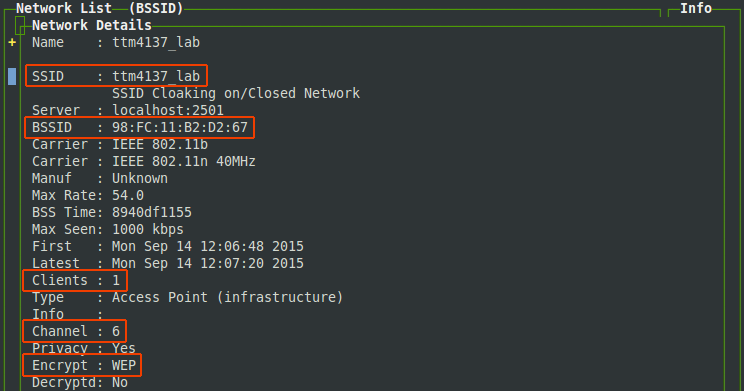
\includegraphics[scale=0.5]{ap_info}}
\caption{\label{fig:kismet}Access Point details found with \texttt{kismet}}
\end{figure}

\begin{figure}[h!]
\centering
\fbox{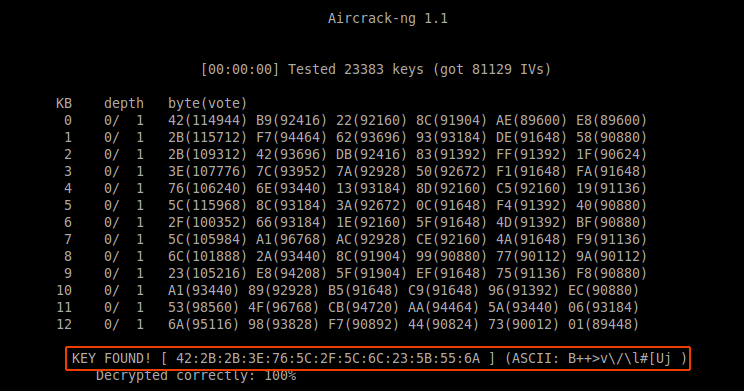
\includegraphics[scale=0.5]{aircrack-ng_key_found}}
\caption{\label{fig:keyfound}Discovering the key with \texttt{aircrack-ng}}
\end{figure}

\noindent\textbf{Q2}. \textit{Is it possible to run a completely passive PTW attack on 104-bit WEP? Why and under which circumstances?} Yes, it is possible to run a passive attack. This requires that there are some client(s) associated with the AP, such that there is some traffic to be captured. It may however take a long time until enough ARP-packets are transmitted across the network. In \cite{ptw}, it is described how IPv4 packets can be used. \\

\noindent\textbf{Q3}. \textit{Why is it possible to send an arbitrary amount of ARP-requests to the AP without knowing the WEP key?} ARP is a link-layer protocol, and (\gls{mac}) addresses are public and can easily be spoofed. Furthermore, WEP does not have a mechanism to detect replay of packets. By capturing one legitimate ARP-request (identified by its characteristic structure), one can replay this multiple times (using e.g. \texttt{aircrack-ng/aireplay-ng}). The AP will accept this packet because the IV/keystream pair is still valid. \\

\noindent\textbf{Q4}. \textit{What can you do to strengthen your attack when there are some clients, but hardly any traffic at all?} As stated in the previous question, one can capture one ARP-request and replay this. Alternatively, is is possible to trick a client to believe that they have been de-authenticated (by sending a \textit{State1}\footnote{If a station is prepared to receive data packets (\textit{State3}), but receives a control packet, it will re-authenticate.} packet), making them re-authenticate with the AP, and thus generate traffic. \\

\noindent\textbf{Q5}. \textit{How can you obtain packets for injection if no clients are associated with the AP?} If no clients are associated with the AP, one can use the following procedure to conduct the attack \cite{noclients}: 1. Fake-authenticate with the AP (using \texttt{aireplay-ng}). 2. Use KoreK's "ChopChop attack" or the "Fragmentation attack" to decrypt a packet in order to obtain the keystream\footnote{Even though no clients are associated, the AP will still transmit some encrypted packets \cite{noclients}.} (ciphertext XOR plaintext). 3. Craft an ARP-request (e.g. using \texttt{packetforge-ng}) and encrypt this with the keystream and IV from the previous step. 4. Inject this multiple times into the network and capture the responses from the AP. 5. Run \texttt{aircrack-ng} when enough packets (IVs) are collected.\\

\noindent\textbf{Q6}. \textit{Which weaknesses of WEP are we taking advantage of in our attack, and why?} \texttt{aircrack-ng} runs the PTW attack by default \cite{aircrack}. This attack extends Klein's attack on RC4, using correlations between the secret key and the generated keystreams to statistically determine the secret key. In addition to this, we take take advantage of WEP's inability to detect packet replays, such that we are able to replay packets at high rates in order to collect large amounts of IVs. \\

\noindent\textbf{Q7}. \textit{Under what circumstances would you consider WEP to be sufficiently secure?} WEP is generally not secure under any circumstances. Only by applying other encryption mechanisms at higher levels (e.g. VPN/IPSec or HTTPS/SSL), we can be confident that our data is not being disclosed to outsiders. Maybe by deploying an advanced \gls{ids} "in-front" of the AP, we can reduce the attack surface (e.g. by detecting ARP injections), but due to the many flaws in WEP, it can never provide sufficient security. \\

\noindent\textbf{Q8}. \textit{Would these attacks be effective against a network deploying WPA with TKIP? If the RC4 cipher used in WEP is considered to be insecure, why is it reused in WPA?} WPA-\gls{wpatkip} is not vulnerable to the same attacks we leveraged against WEP. For one, the \textit{Root/Master key} is not used to encrypt traffic. A new key is generated for each packet. Also, the IV is used as a packet counter, prohibiting replay of packets. The reason RC4 is still used in WPA is that it was only developed as a so-called "stopgap" protocol in order to patch the most critical vulnerabilities of WEP \cite{wepwiki}, as the hardware in the existing APs did not support any other encryption algorithms. 

\section{Password Dictionary Attack} 

The second part of the lab consisted in running a brute-force dictionary attack against a WLAN running \gls{wpa}-\gls{psk}, in order to determine the secret password. This password is the basis for all confidentiality in the WPA-PSK protocol, thus discovering this could be considered a major security breach. In order to check if we are guessing correctly, the password and other network specific parameters must be fed into two different key derivation functions (parameters listed in \textit{Q10} below). Two of these parameters can only be obtained during the authentication procedure (4-way handshake) between the supplicant and AP.

\subsection{Lab Set-up}

We used the following set-up for this part:

\begin{description}
	\item[Lab Computer 1] Using \texttt{hostapd}, we set up a WLAN AP, running WPA-PSK, on the wireless NIC. We also we set up a bridge between the NIC and the Ethernet port for Internet access. SSID: \textit{TheMatrix}, password: \textit{Garden01}.
	\item[Lab Computer 2] Running packet capture with \texttt{airodump-ng} to catch the 4-way handshake, and then execute the brute-force dictionary attack.
\end{description}

\noindent See \nameref{sec:appendixb} for all the changes we made in the \texttt{hostapd.conf} file.

\subsection{Attack Procedure}

\textbf{Password dictionary}: To set up our dictionary for the attack, we first needed a list of words that we could extend to match typical password patterns. We chose a word list with approximately 28 000 English words \cite{wordlist}. To create different variations of each word we used the tool \texttt{John the Ripper}. We modified the \texttt{john.conf} file to adapt to the rules to our case \cite{johnrules}. The following command takes in a list \texttt{lower.lst} that contains the words we want to use as a basis for our dictionary. \texttt{-stdout -rules} applies the rules we defined in john.conf to all the words in lower.lst and outputs it to \texttt{extendedwords.lst}: \texttt{john --wordlist=lower.lst --stdout --rules > extendedwords.lst}\\

\noindent \textbf{De-authentication}: We then connected a smartphone to our network. We started \texttt{airodump-ng} to capture the traffic on our network.  We used \texttt{aireplay-ng} to de-authenticate the connected device so we could capture the 4-way handshake once it reconnected. This was necessary in order to get the \texttt{ANonce} and \texttt{SNonce}. It is important to note that this step is not required, as you may just simply wait until a client connects to the network to capture these parameters, making this attack completely passive. \\

\noindent \textbf{Cracking the password}: The final step was to run \texttt{aircrack-ng} with our captured file, password dictionary and the SSID. Thus, the only unknown value was the password. We ran \texttt{aircrack-ng} with the following parameters: \texttt{-a wpa}, meaning that we are attacking WPA, \texttt{-b} denoting the \texttt{BSSID}, \texttt{-w} for  the word list we used, and fileCapture.cap was our traffic dump from \texttt{airodump-ng} \cite{aircrack}: \texttt{aircrack-ng -a wpa -b TheMatrix
-w extendedwords.lst fileCapture.cap}

\begin{figure}[h!]
\centering
\fbox{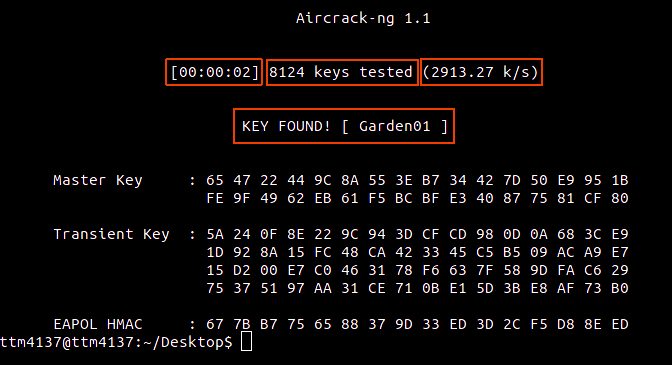
\includegraphics[scale=0.5]{wpakey}}
\caption{\label{fig:result2} Result from running the dictionary attack with \texttt{aircrack-ng}}
\end{figure}

\subsection{Results}

\noindent We experienced the big drawback with brute-force attacks. After 30 minutes of wrong guesses, we decided to remove some rules from our \texttt{john.conf} file, in order to make it feasible to complete the lab within our lab hours, and confirm that our setup worked. In the second run, we were "lucky" to find the key after \textbf{8,124} tested keys. As shown in figure \ref{fig:result2}, the lab computer was able to test approx. 3,000 keys per second, and so the key was found within \textbf{3 seconds}. Considering that we had drastically reduced the password space for the second run, we acknowledge the fact that brute-force attacks may be very time-consuming.

\subsection{Questions}

\noindent\textbf{Q9}. \textit{Why is TKIP a more secure encryption mechanism than the one-key WEP alternative?}
\noindent TKIP was introduced as a intermediate solution in the mitigation process from WEP to what is now known as WPA2. WEP's major drawback is the fact that all devices on the same network use the same key to encrypt their data. WPA introduced improved key management through TKIP. It scrambles the keys with a hashing algorithm and adds a \gls{mic}. With TKIP, each wireless client have unique encryption keys, which are constantly changed\cite{iee802}.\\

\noindent\textbf{Q10}. \textit{Which information is used to compute the Pairwise Master Key (PMK) and the Pairwise Temporary Key (PTK) in the password-based PSK scenario? Why is the offline password brute-force attack possible?} The PMK is calculated as follows: \[PMK = PSK = \gls{pbkdf}(\: password, SSID, SSID_{length}, Hash_{count}, Output_{length}\:) \]
In this example the pairwise master key is equal to the pairwise session key which is calculated from the password and the SSID of the wireless network. The last two parameters determine the number of hashes/rounds and the length of the output. The \gls{ptk} is calculated as: \[ PTK = f(PMK, MAC_{AT}, MAC_{STA}, Nonce_A, Nonce_S) \]
\noindent The offline brute force attack is possible because the initial 4-way handshake is done in plain text. This makes it possible for an attacker to pick up MAC addresses and nonces. These values are all that is needed in order to start guessing the PSK offline. \\

\noindent\textbf{Q11}. \textit{Does the compromise of password imply the disclosure of traffic from previous sessions? Justify your answer.} Under the circumstances that an attacker have been capturing all traffic since the initial handshake (which can be provoked by a deauthentication attack), he or she will have all the required information in order to calculate the PTK, which is used to encrypt the traffic within the current session. However, if the captured data spans multiple sessions, they may have to re-calculate the PTK for each session (with unique nonces for each session).\\

\noindent\textbf{Q12}. \textit{Does the use of AES in WPA2-PSK give an advantage against a password dictionary attack, as compared to RC4 in WPA-PSK?} No, the encryption algorithm does not matter because the dictionary attack only targets the 4-way handshake, where encryption is not yet applied. \\

\noindent\textbf{Q13}. \textit{What would be advantages and disadvantages of using a pre-computed database of PMK in a PSK password dictionary attack?} The PMK is computed as PMK = PSK. The PSK is a key derived (through PBKDF2) from the password and the SSID of the network. Because SSIDs usually are different, a so called "rainbow table" of pre-computed hashes wouldn not give any advantage, as you would have to pre-compute these tables for every SSID. What you could do however, is to pre-compute these hashes for common SSIDs, but that would require a tremendous amount of time/resources, which might turn out to be a waste of time.\\

\noindent\textbf{Q14}. \textit{Suppose an attacker employs 30 days of processing time on the new supercomputer at NTNU. Which minimum requirements would you put on a WPA password to ensure that the probability of successful attack does not exceed 2e-20?} In our lab we put pretty hard constraints on our password, restricting it to only consist of upper- and lowercase letters and numbers. This is makes up 62 unique ASCII characters, and for this calculation we wanted to find out how long our key had to be in order to be within the an acceptably low probability of being compromised. We concluded that our password had to be \textbf{at least 15 characters long}. A justification and the full calculations can be found in \nameref{sec:appendixc}.

\section{Setting up RSN-EAP Wireless Access Point}

This challenge was not about \emph{attacking} an insecure network, but rather \emph{defending} by setting up a secure network. The main objective was to set up a wireless access point and configure it's security features following industry standards. Part 2 of the lab demonstrated the weaknesses with the handshake in WPA-PSK. In order to mitigate this and establish mutual authentication of both the supplicant and the authentication server we employed CCMP, the EAP-TLS authentication protocol and digital certificates based on public key encryption. The following section will address the the necessary steps in order to achieve this, before discussing how and why this is a secure setup.

\subsection{Lab Set-up} % (fold)
\label{sub:lab_set_up}
% subsection lab_set_up (end)asdfasd

For challenge 3 the we used three computers which were allocated the following responsibilities:
\begin{description}
	\item[Lab Computer 1] Certificate Authority (\gls{ca}), responsible for generating and signing certificates for all entities.
	\item[Lab Computer 2] Authentication Server (\gls{as}) running FreeRadius and serving as an AP and Authenticator configured with \texttt{hostapd}.
	\item[Personal Computer] Supplicant with a personal certificate. Sole responsibility was to connect to the secure access point. 
\end{description}

\subsection{Configuration Procedure} % (fold)
\label{sub:configuration_procedure}

\textbf{Setting up the CA}: Starting with the certificate authority, we used the OpenSSL software in order to create a private key and certificate for the CA. This certificate was self-signed, meaning this CA now would be a \emph{Root Certificate Authority} \cite{rootca} for everyone it should issue certificates to. We downloaded an \texttt{openssl.conf} template file \cite{openssl-conf} and changed default values to something suitable for our little CA organisation, as well as the key length (2048 bit) and message digest algorithm (sha256) to values that are considered secure at the moment \cite{cookbook}. 

Creating and self-signing a certificate can all be done with the following one-liner: \texttt{openssl req -new x509 -keyout cakey.pem -out cacert.pem -config ./openssl.cnf}. The \texttt{req -new -x509} flags tell OpenSSL that we want to create a X.509 Certificate Signing Request (CSR) and sign it. The output is two \texttt{.pem} files, which contain the self-signed (root) certificate (see \nameref{sec:appendixd}) and the CA's private key. This key is protected by a password, created at the same time. We then went on and created private keys and certificates for the supplicant and AS: \texttt{openssl req -new -out supplicantreq.pem -keyout supplicantkey.pem -config ./openssl.cnf} (repeated for the AS with new file names). \\

\noindent \textbf{Note:} The lab notes instructed us to create all certificate related files (including public/private key pairs) on one machine and then transfer it to the other actors later. No one should \emph{ever} generate nor handle your private key. It is important to note that outside the lab, both keys and certificates should be generated locally, and then the certificate can be sent to the CA for signing.\\

\noindent The two certificates were then signed by the CA, once again with the OpenSSL terminal program: \texttt{openssl ca -out supplicantcert.pem -config ./openssl.cnf -infiles supplicantreq.pem} (and again the same for the AS). We then transferred the files to the respective computers with a USB stick. \\

\noindent\textbf{The authentication server}: In order to set up the AS, we used the FreeRadius program. The program has a lot of default settings, and we modified two files, \texttt{eap.conf} and \texttt{clients.conf}, located in \texttt{/etc/freeradius}. In the \texttt{eap.conf} file (\nameref{sec:appendixe}) we specified the absolute path to where our certificates and keys were located. Another input for the AS is a file containing parameters for the Diffie-Hellman key exchange, along with a file containing random bytes. These two files can be created with the following commands: \texttt{openssl dhparam -out dh 1024} and \texttt{openssl dhparam-out random 256}. We also made sure that the default EAP method was set to TLS. 

In the \texttt{clients.conf} file we had to specify who was going to communicate with the AS. In our case the AP and AS were located one same machine. Therefore, we made sure \texttt{localhost} was the only client that was "uncommented". We also set a shared secret between the AS and the AP. We then started the server with the \texttt{freeradius -X} command. \\

\noindent \textbf{Note:} We encountered some permission problems when first firing up the FreeRadius server. The server is configured to run with it's own user, which in our case did not have read access to the certificate files. We solved this by changing ownership of all the certificate files   \texttt{chown -R freerad:freerad ../CA/}. \\

\noindent\textbf{Access point}: The AP would act as a mediator between the supplicant and the AS, as well as handling encryption CCMP for the wireless communication. These configurations were done in the \texttt{hostapd.conf} file (see \nameref{sec:appendixf}). \\

\noindent\textbf{Connecting to the network}: The easiest way of connecting to the network was to use our operating system's built in network connection manager. After finding the wireless network in the list of available networks, we had to locate the certificates we received from the CA via USB and specify both the CA certificate and our own along with our private key with its password. Any value is accepted in the the identity field, so after this we were able to connect to the RSN with link layer encryption (see \nameref{sec:appendixg}).

\subsection{Results} % (fold).

We successfully set up an RSN with AES-CCMP link encryption and mutual authentication.

\label{sub:results}

% subsection results (end)

\subsection{Questions}

\textbf{Q15}. \textit{When would it be appropriate to use WPA2-PSK instead of WPA2-EAP (as a key management scheme)?} It would be better to use in small environments where there are not too many users, where it is easier to keep an overview over the people on the network and thus individual authentication can seem unnecessary. The issue with using a PSK is that everyone use the same key, and that increases the risk of the key being compromised. This is why it should be used with few users to limit the chances of this happening, and make it easy to change if it would happen. \\

\noindent \textbf{Q16}. \textit{\gls{eap}-\gls{tls} deploys mutual authentication of two communicating parties. What kind of attack is possible against authentication protocols lacking such authentication?} \gls{mitm} attack could be possible if there is no mutual authentication. The typical scenario would be that the user authenticates to the server, but the server does not authenticate to the user (as in e.g. GSM). This could allow for an attacker to set up a fake AP and possibly disclose sensitive information, hijack the traffic, or tamper with the packets. Considering if the client is not authenticated, an attacker could impersonate a legitimate client act maliciously on their behalf. \\

\noindent \textbf{Q17}. \textit{Give an overview of the \gls{eap} authentication protocols which can be used in WPA2- Enterprise WLANs.} The following protocols can be used \cite{wpawiki}:

\begin{description}
\item [\gls{eap}-\gls{tls}]The original standard in wireless security.

\item [EAP-\gls{ttls}/\gls{mschap}v2] Creates a secure tunnel before starting authentication.

\item [PEAPv0/EAP-MSCHAPv2] Also uses a secure tunnel to protect the authentication.

\item [PEAPv1/EAP-\gls{gtc}] Uses a text challenge and securtiy token for authentication.

\item [EAP-\gls{sim}] A SIM-card is used for authentication.

\item [EAP-\gls{aka}] Used in \gls{umts}.

\item [EAP-\gls{fast}] Uses \gls{pac} to create a secure TLS tunnel where a client can be verified.
\end{description}

\noindent\textbf{Q18}.\textit{ List the security-related protocols used in your RSN-EAP-TLS setup and explain their purpose.} \textbf{EAP} - Provide functions and methods for authentication protocol transport, without IP connectivity. \textbf{TLS} - Used to negotiate a symmetric key for transport between the communicating endpoints. It ensures confidentiality and integrity. \textbf{\gls{radius}} - Is used for the communication between the Authenticator (AP) and AS. It runs on the application layer. It is used to grant or deny access to the network. \textbf{\gls{ccmp}} - Is used to encrypt the data sent over the wireless network. It guarantees authenticity, integrity and confidentiality. It uses AES with counter mode cipher block chaining. It provides data confidentiality, authentication. \textbf{\gls{rsn}/WPA2} - The latest security standard in wireless security. Its purpose is to secure wireless computer networks. It is the replacement for WPA that used temporal keys. WPA2 has mandatory support for CCMP mentioned above. What separates it from WPA is the encryption and key management.\\

\noindent\textbf{Q19}. \textit{How can this lab project be improved?} We were satisfied with how the lab was organized, and the lab description was very helpful. There was only one issue with the configuration in part 3, where some parameters for \texttt{eap.conf} and \texttt{client.conf} were left out, and this did cause some confusion to why the setup did not work at first. Also we would have preferred if the answers to the questions could be "merged" into the report, instead of being a separate part. In some situations, we had to choose between repeating an answer to a question, or leaving it out where it seemed natural to mention it.

\begin{thebibliography}{9}

\bibitem{thebook}
Jon Edney and William A. Arbaugh.
\emph{Real 802.11 security: Wi-Fi protected access and 802.11i},
Boston, MA: Addison-Wesley 2004 ISBN: 0-321-13620-9.

\bibitem{wepwiki}
Wikipedia: The Free Encyclopedia, Wikimedia Foundation Inc.
"Wired Equivalent Privacy",
\emph{en.wikipedia.org/wiki/Wired\_Equivalent\_Privacy}.
Visited 21 September 2015.
  
\bibitem{ptw}
Erik Tews, Ralf-Philipp Weinmann and Andrei Pyshkin.
\emph{Breaking 104 Bit WEP in Less Than 60 Seconds},
TU-Darmstadt, FB Informatik.
  
\bibitem{noclients}
Aircrack-ng.org.
"Tutorial: How to crack WEP with no wireless clients",
\emph{www.aircrack-ng.org/doku.php?id=how\_to\_crack\_wep\_with\_no\_clients},
Version 1.16 (darkAudax).
Visited 22 September 2015.

\bibitem{aircrack}
Aircrack-ng.org.
"Aircrack-ng Description",
\emph{www.aircrack-ng.org/doku.php?id=aircrack-ng}.
Visited 22 September 2015.

\bibitem{johnrules}
OpenWall.
"Rules for john the ripper config file"
\emph{www.openwall.com/john/doc/RULES.shtml}.
Visited 24 September 2015.

\bibitem{wordlist}
OpenWall.
"List of English words in lower-case (lower.gz)",
\emph{ftp.openwall.com/pub/wordlists/languages/English/1-tiny/}.
Visited 19 September 2015.

\bibitem{wpawiki} 
Wikipedia: The Free Encyclopedia, Wikimedia Foundation Inc.
"Wi-Fi Protected Access",
\emph{en.wikipedia.org/wiki/Wi-Fi\_Protected\_Access}.
Visited 21 September 2015.

\bibitem{openssl-conf}
Eclectica.
"Creating and Using SSL Certificates",
\emph{www.eclectica.ca/howto/ssl-cert-howto.php}.
Visited 23 September 2015.

\bibitem{cookbook}
Ivan Ristić.
OpenSSL Cookbook / SSL/TLS Deployment Best Practices,
Feisty Duck, Qualys.
Available at \emph{https://www.feistyduck.com/books/openssl-cookbook/}.
Visited 26 September 2015.

\bibitem{ascii}
Wikipedia: The Free Encyclopedia, Wikimedia Foundation Inc.
"ASCII Printable Characters",
\emph{en.wikipedia.org/wiki/ASCII\#ASCII\_printable\_characters}.
Visited 23 September 2015.

\bibitem{fjord}
NTNU HPC GROUP / Vilje.
"About Vilje",
\emph{www.hpc.ntnu.no/display/hpc/About+Vilje}.
Visited 23 September 2015.

\bibitem{rootca}
Microsoft Technet.
"Certification Authority Trust Model",
\emph{technet.microsoft.com/en-us/library/cc962065.aspx}.
Visited 23 September 2015.

\bibitem{vilje}
NTNU.
"The Norwegian University of Science and Technology, met.no buy new supercomputer",
\emph{www.ntnu.edu/news/new-supercomputer-to-be-installed}.
Visited 23 September 2015.

\bibitem{flops}
Wikipedia: The Free Encyclopedia, Wikimedia Foundation Inc.
"Floating Point Operations Per Second",
\emph{https://en.wikipedia.org/wiki/FLOPS}.
Visited 26 September 2015.

\bibitem{iee802}
Wikipedia: The Free Encyclopedia, Wikimedia Foundation Inc.
"IEEE 802.11i-2004",
\emph{https://en.wikipedia.org/wiki/IEEE\_802.11i-2004}.
Visited 27 September 2015.


\end{thebibliography}

\newpage

\section*{Appendix A} \label{sec:appendixa}

\printglossaries

\section*{Appendix B} \label{sec:appendixb}
Changes made to \texttt{hostapd.conf} file to set up our WPA-PSK WLAN AP in part 2 of the assignment. \\

\begin{tabular}{ll}
\texttt{ssid = TheMatrix} & Setting the SSID \\https://www.sharelatex.com/project/56053f240a0801262694cf16
\texttt{wpa = 1} & Enabling WPA\\
\texttt{wpa\_passphrase = Garden01}  & Setting the secret key (to be cracked)\\
\end{tabular}

\section*{Appendix C} \label{sec:appendixc}
In order to calculate the probability of a successful attack, we first have to look at NTNU's supercomputer and it's capabilities. The article referenced \cite{fjord} in the Lab Description says Vilje will be able to do 275 trillion floating point operations per second. Updated numbers \cite{vilje} reveal that the hardware has been upgraded since 2011, and Vilje should now be capable of ~397 Teraflops/s. There are multiple approaches as to how to determine the number of keys that can be tested per second given a number of FLOPS. Our lab machine peaked at 3000 guesses per second, and they run at 2.5Ghz processors. However, it is reasonable to assume that Vilje is optimised for operations like this both in hardware and in OS/software, so for the sake of the calculation we assume that Vilje would require 10 floating-point operations to check one key (see \cite{flops}). This lets us test \[
	\dfrac{397\: e^{12}}{10}\: flops\: \times\: 2592000\: seconds = 1.02\: e^{20}
\] number of keys in 30 days. The WPA passphrase is limited to 63 printable ASCII characters \cite{ascii}, and has to be at least 8 characters long. Further, the IEEE Standard (802.11i-2004, Annex H.4.1) specifies the characters to have an encoding in the decimal range of 32 to 126. Given a uniform random distribution among all of the characters, this gives us 95 different symbols to work with on up to 63 characters. In our lab we put pretty hard constraints on our password, restricting it to only consist of upper- and lowercase letters and numbers. This is makes up 62 unique ASCII characters, and for this calculation we want to find out how long our key has to be in order to be within the an acceptably low probability of being compromised: 
\[
	p = \frac{keyschecked}{num\: of\: possible\: keys} = \frac{1.02\: e^{20}}{62\: ^x}\: \leq\: 2^{-20}\: 
\] this gives us,
\[
	log\bigg(\: \frac{1.02\: e^{20}}{2^{-20}}\: \bigg)\: \leq\: log(62^x)\:\: which\: is,\:\: log\bigg(\: \frac{1.02\: e^{20}}{2^{-20}}\: \bigg)\: \leq\: x\times log(62)
\] and finally,
\[
	x \geq \frac{log\Big(\: \frac{1.02\: e^{20}}{2^{-20}}\: \Big)}{log(62)} = 14.522 \approx 15
\]

\noindent This means our password has to be \textbf{at least 15 characters} long, if we are only using upper and lowercase characters and numbers.

\newpage

\section*{Appendix D} \label{sec:appendixd}
The root certificate used in part 3 of the assignment: \\

\begin{figure}[h!]
\centering
\fbox{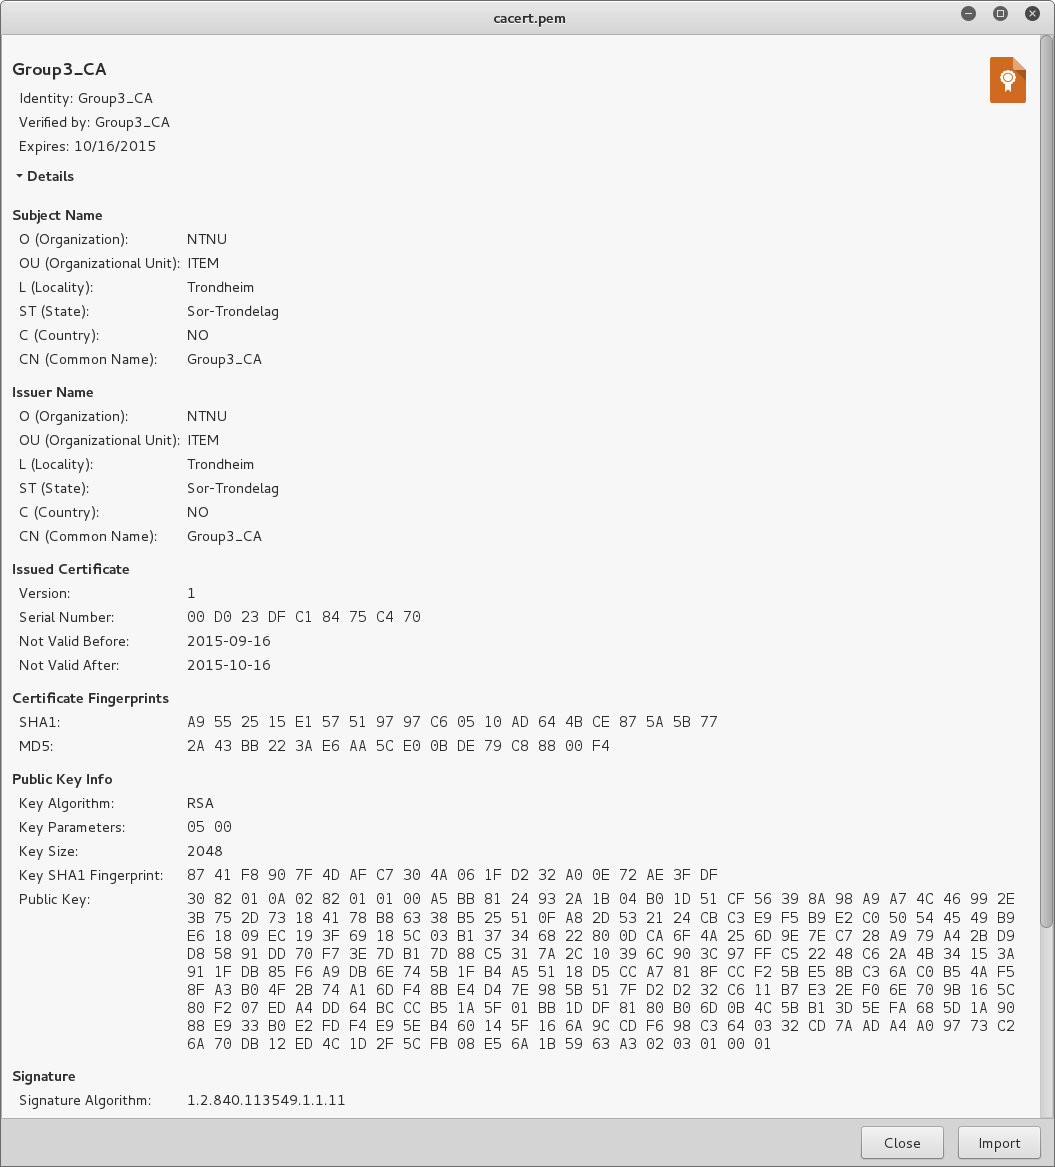
\includegraphics[scale=0.4]{cacert}}
\caption{\label{fig:rootcert} Screenshot of our self-signed root certificate}
\end{figure}

\newpage

\section*{Appendix E} \label{sec:appendixe}
Changes made to \texttt{eap.conf} in \texttt{/etc/freeradius/} in part 3 of the assignment. \\

\noindent\texttt{\#TLS}\\
\texttt{certdir = /home/ttm4137/Desktop/CA/newcerts} \\
\texttt{cadir = /home/ttm4137/Desktop/CA} \\
\texttt{private\_key\_password = birkeland} \\
\texttt{private\_key\_file = \${cadir}/private/askey.pem} \\
\texttt{certificate\_file = \${certdir}/ascert.pem} \\

\noindent\texttt{\#Trusted Root CA list} \\
\texttt{CA\_file = \${cadir}/cacert.pem} \\
\texttt{dh\_file = \${certdir}/dh/dh} \\
\texttt{random\_file = \${certdir}/dh/random} \\

\section*{Appendix F} \label{sec:appendixf}
Changes made to \texttt{hostapd.conf} file to set up our WPA2-EAP-TLS WLAN AP in part 3 of the assignment. \\

\begin{tabular}{ll}
\texttt{ieee8021x = 1} & Enabling 802.1X \\
\texttt{wpa = 2} & Enabling IEEE 802.11i/RSN (WPA2)\\
\texttt{wpa\_key\_mgmt = WPA-EAP}  & Key management \\
\texttt{wpa\_pairwise = CCMP}  & Encryption mechanism \\
\texttt{auth\_server\_addr = 127.0.0.1} & AS (RADIUS) address, localhost \\
\texttt{auth\_server\_shared\_secret = gunnar} & Shared secret between AP and AS.
\end{tabular}

\newpage

\section*{Appendix G} \label{sec:appendixg}

Connecting to the RSN.

\begin{figure}[h!]
\centering
\fbox{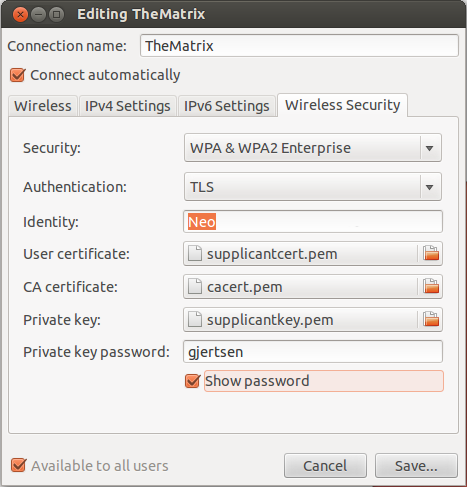
\includegraphics[scale=0.5]{eapcert}}
\caption{\label{fig:eapclient} Client-side connection interface.}
\end{figure}

\begin{figure}[h!]
\centering
\fbox{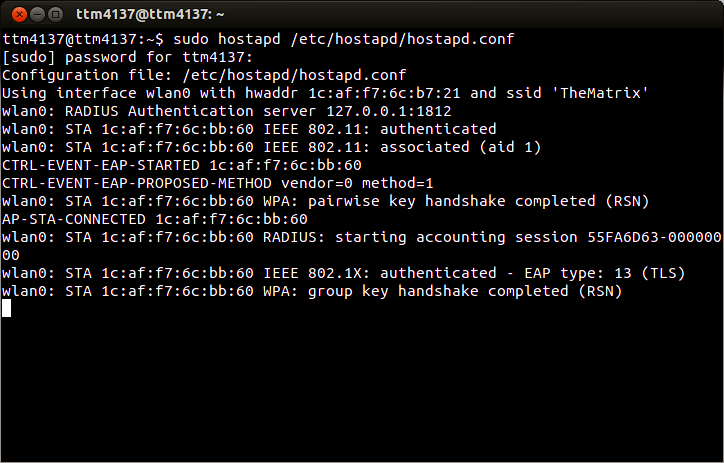
\includegraphics[scale=0.5]{handshake}}
\caption{\label{fig:eap4way} Screenshot from the AP. Authentication successful.}
\end{figure}

\end{document}